\subsection{Region Transition Probability}
For event distribution of the load and drop events are different with each other and varied with time, the region $R_{i,t}^{load}$ and $R_{j,t}^{drop}$ are recognized by different metrics, that is, drop or load event distribution during  each time period. For instance, if the taxi is currently occupied, then the next hop event is the drop one. Hence, choosing a target region from a region set obtained based on drop event distribution is more logical. 

Before defining the region transition probability, we first describe our \textbf{region recognition process}.
Firstly, we divide the area into small grids of side length 200 meters, and define them as cells (as shown in the following equation) where $lon$ and $lat$ are relevant longitude and latitude, $X$ and $Y$ are side length of the grid/cell).
\[C_{x,y}::=\{(lon,lat)|x \le \frac{{lon}}{{X}} < x + 1,
y \le \frac{{lat}}{{Y}} < y + 1\}.\]
Then, we consider a region as a union of adjacent cells, as following.
\[R_m:: = \{ C_{i,j}|if C_{x,y} \in R_m
\Rightarrow \|x - i\| \le 1,\|y - j\| \le 1\}.\]
$m$ denotes the region identifier.
The main idea of clustering cells to regions is merging adjacent cells whose event density is larger than an event threshold $\eta$ into a same region.
For drop/load event, this process is conduct respectively. 
Three parameters, threshold $\eta$, Cluster Size and range $\_top$, are used in this process. 
Cluster Size defines the size of region, i.e., it is a limitation on the size of a region, saying $\|R_i\|\leq ClusterSize$.
We only consider the top $_top$ regions, in which event density of each cells are larger than threshold $\eta$.
For each time period,  we set different threshold by its average events number in each cell at that time, that is, $\eta$ equals to twice the average event number.

\begin{table}
\caption{region recognization parameters}
\centering
\begin{tabular}{l|c|c|c|c}
  \hline
  Item & 0:00-8:59 &9:00-12:59&13:00-20:59 &21:00-23:59 \\
  \hline
  $\eta_{drop}$ & 56&84 &180 &51\\
  $\eta_{load}$ & 58&84 &182 &51\\
  \_top & 200&200 &200 &200\\
  clusterSize& 500&500 &500 &500\\
  \hline
\end{tabular}
\end{table}

The overall clustering algorithm is shown as follows. We sort the all the cells by event density in descending order, 
and begin with the first cell to search its neighbors whether to join the same region or not using breadth traversal. 
After the top regions are formed, the other cells which do not belong to the top \_top regions will also be clustered into regions, 
whose size should still be small than Cluster Size. Consequently, every cells will be clustered into regions and the size of each region are not larger than Cluster Size.
By clustering cells into regions, two region sets, \textbf{$R^{load}$} and \textbf{$R^{drop}$}, can be recognized from the data set for every time period. As can be seen from Fig. \ref{figure_region_recognizition}, the differences among load region and drop regions for the Beijing taxi data set are clear.
In this figure, every colored block presents a region.In addition, Cluster Size = 200, range t = 200 (range is the same with Cluster Size by coincidence) and threshold $\eta = 121$ are set for load event and $\eta$ equates with 141 for drop event (these are set by the average event density of the top 5000 cells order by its event density).

\begin{figure}[!t]
\centering
\subfigure[drop event regions]{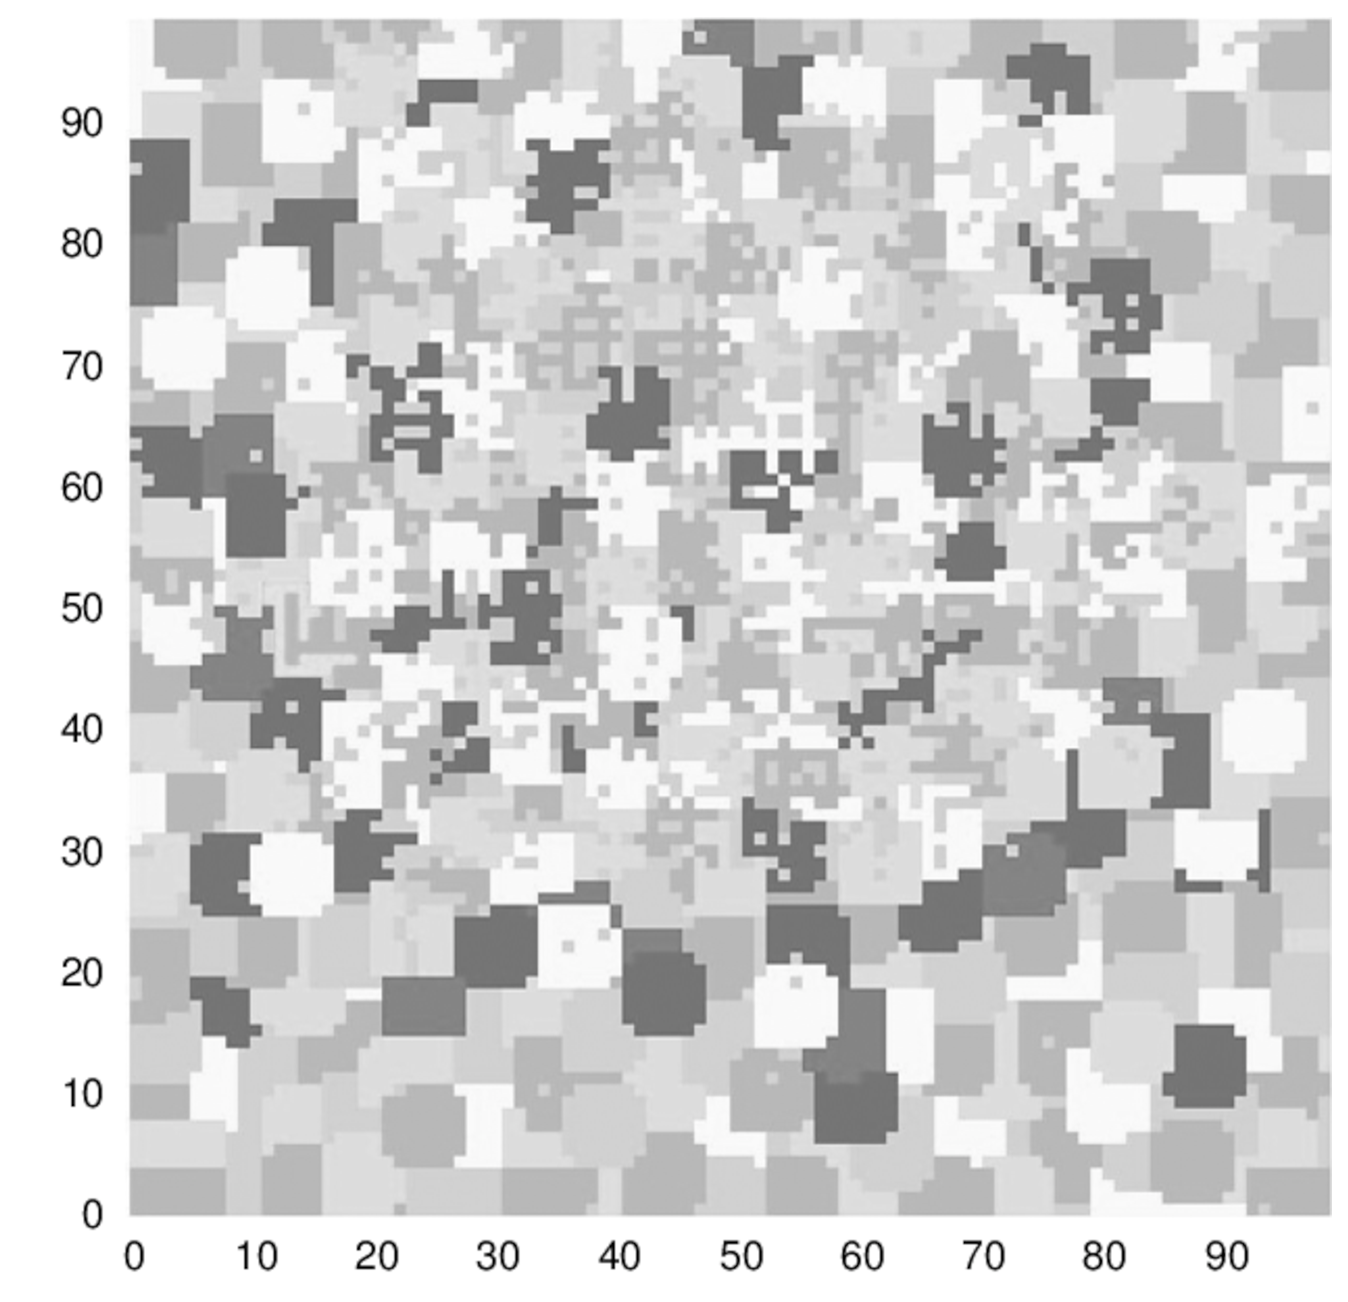
\includegraphics[width=0.23\textwidth]{figures/region/Areas-2011_event01.eps}}
\subfigure[load event regions]{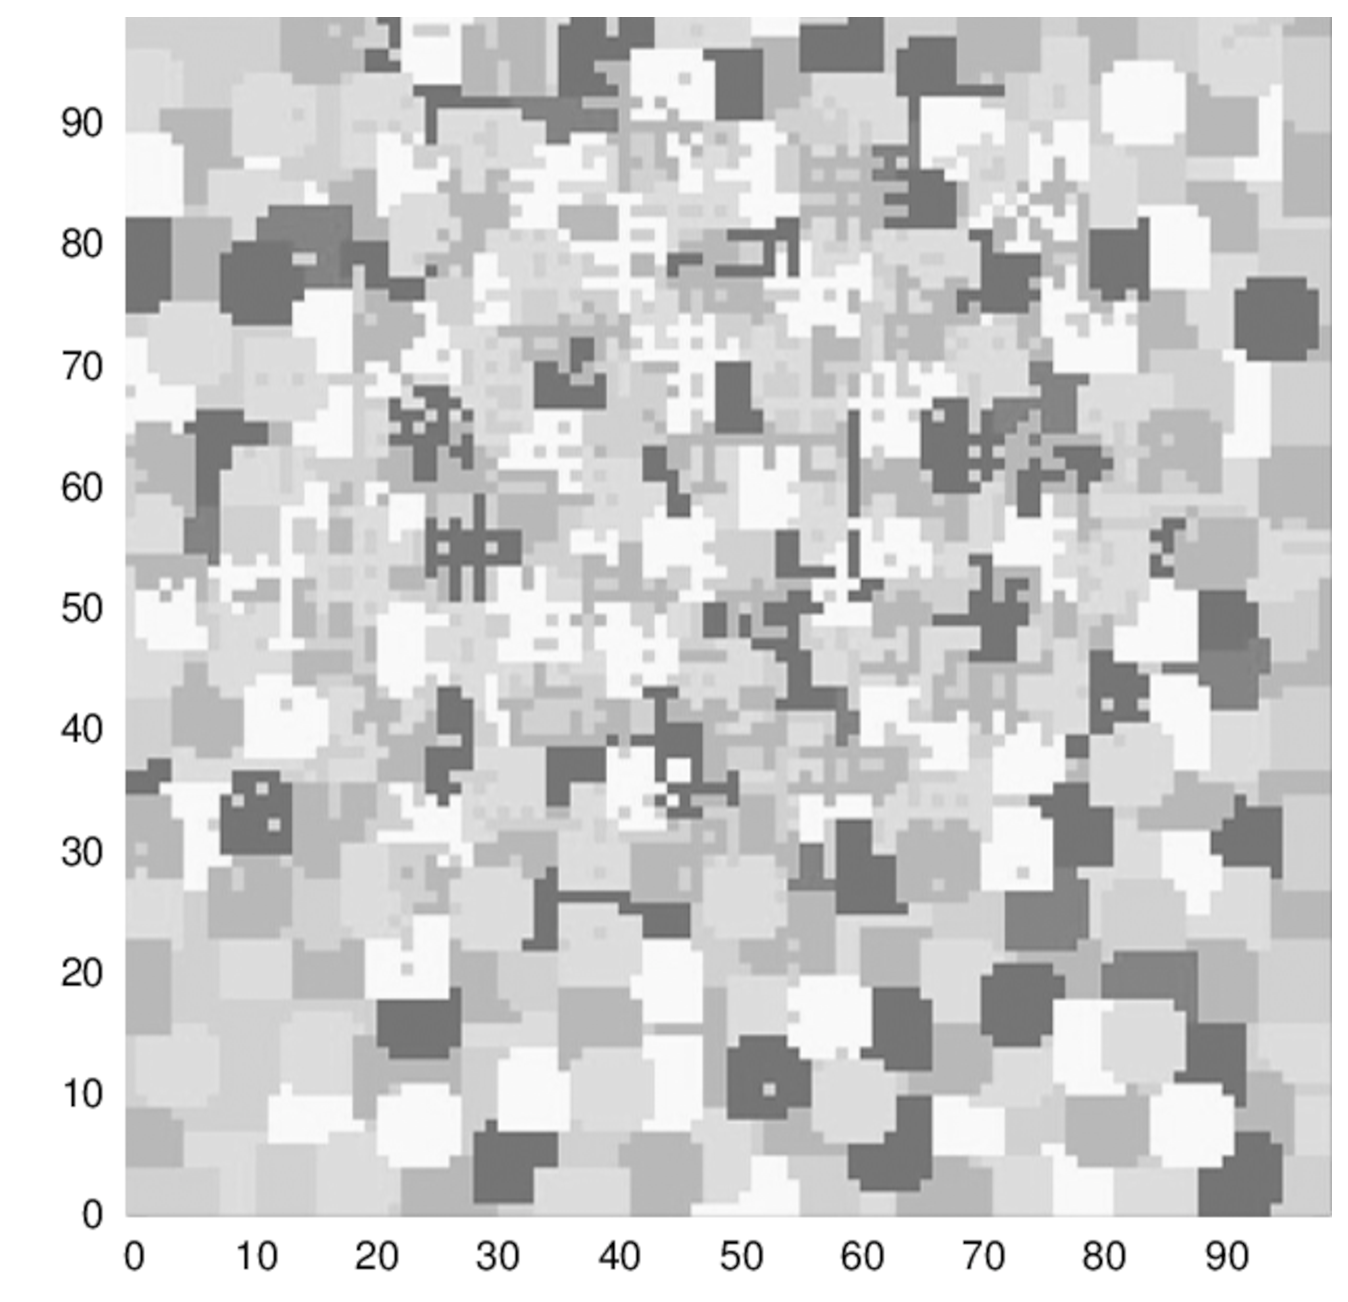
\includegraphics[width=0.23\textwidth]{figures/region/Areas-2011_event03.eps}}
\centering
\caption{Region recognition}\label{figure_region_recognizition}
\end{figure}

\textbf{Calculation of region transition probability}:
we define a region transition probability to figure out the probability of the next hop falling in a certain region from the current region.  A transition probability from a load region i to a drop region j from time t is denoted as:
\begin{equation}
p^{load\rightarrow drop}_{i\rightarrow j,t}
\end{equation}
Similarly, A transition probability from a drop region j to a load region i from time t is denoted as:
\begin{equation}
p^{drop\rightarrow load}_{j\rightarrow i,t}
\end{equation}


 After clustering cells into regions, the transition probability from $R_i^{load}$ to $R_j^{drop}$ and the one from $R_i^{drop}$ to $R_j^{load}$, donated as $p_{i\rightarrow j}^{load\rightarrow drop}$ and $p_{i\rightarrow j}^{drop\rightarrow load}$, can be caculated. Since both transition probability can be calculated similarly, we only introduce the detailed one of $p_{j\rightarrow i}^{drop\rightarrow load}$.

To calculate a $p^{drop\rightarrow load}_{j\rightarrow i,t}$, we should find out all the taxies in the drop region j of time t, denoted as $V^{drop}_{j,t}$. For every taxi $v \in V^{drop}_{j,t}$ , its next load event record, which marks where when it load passengers, can be extracted. 	we map every next load event records to according region of corresponding time range and find out how many records fall in the region i. The transition probability equals to the ratio between the total taxies  and the amount of taxies whose next load events happen in region i.
We restrict the time from current drop event record to next load event cannot be across more than one hour, that is the region i belongs to the region set of time t or time $t+1$ and we ignore the records whose hour of timestamp is more than $t+1$ hour. For example, for $t=7$,  the record with timestamp 9:00:00 is invalid, while the record whose timestamp is 8:59:59 is valid.
The method to calculate a $p^{load\rightarrow drop}_{i\rightarrow j,t}$  is similar. 
